\documentclass{beamer}
\usepackage[utf8]{inputenc}
\usepackage[main=spanish]{babel}

\usetheme{Madrid}
\useoutertheme[subsection=false]{miniframes}
\usecolortheme{default}

\uselanguage{spanish}
\languagepath{spanish}
\deftranslation[to=spanish]{Lemma}{Lema}
\deftranslation[to=spanish]{Theorem}{Teorema}

\setbeamertemplate{caption}[numbered]


\usepackage{nicefrac}
\usepackage{tikz}

% --- Configuración de enlaces ---

\let\originalhref\href
\renewcommand{\href}[2]{\originalhref{#1}{\color{blue}\ul{#2}}}

% --- Configuración de bibliografía ---
\usepackage[backend=biber]{biblatex} % 'style' puede ser numeric, alphabetic, etc.
\addbibresource{Bibliografia.bib} % Tu archivo de citas (.bib)



\newcommand{\bb}[1]{\mathbb{#1}}
\newcommand{\cc}[1]{\mathcal{#1}}
\newcommand{\ul}[1]{\underline{#1}}
\DeclareMathOperator{\diag}{diag}


\setbeamercolor{bloqueAmarilloCc}{bg=orange!90!yellow, fg=white} % Cabecera
\setbeamercolor{bloqueAmarilloCu}{bg=orange!6!yellow!4!white, fg=black} % Cuerpo

\newenvironment{definitionblock}[1]{%
  \begin{beamerboxesrounded}[upper=bloqueAmarilloCc, lower=bloqueAmarilloCu, shadow=true]{#1}%
}{%
  \end{beamerboxesrounded}%
}


\AtBeginSection[]
{
  \begin{frame}
    \frametitle{Índice}
    \tableofcontents[currentsection]
  \end{frame}
}


% Declarar aplicaciones
% 1. Nombre aplicación
% 2. Dominio
% 3. Codominio
% 4. Variable
% 5. Imagen de la variable
\newcommand{\Func}[5]{
    \begin{equation*}
        \begin{array}{rrll}
            \displaystyle #1:& \displaystyle  #2 & \longrightarrow & \displaystyle  #3\\
               & \displaystyle  #4 & \longmapsto & \displaystyle  #5
        \end{array}
    \end{equation*}
}
\DeclareMathOperator{\tr}{Tr}


\usepackage[makeroom]{cancel}


\title[2.2. DDPM]{Capítulo 2.2. Denoising Diffusion Probabilistic Models}
\subtitle{Trabajo de Fin de Grado}
\author[Arturo]{Arturo Olivares Martos}
\institute[DGIIM - UGR]{Doble Grado en Ingeniería Informática y Matemáticas\\Universidad de Granada}
\date{\today}
\logo{
\includegraphics[height=1cm]{Aux/UGR-Logo.png}}

\usetikzlibrary{positioning, shapes.geometric, arrows.meta, calc}



\begin{document}

\begin{frame}
    \titlepage
\end{frame}

\section{Introducción}
\begin{frame}
    \frametitle{Denoising Diffusion Probabilistic Models}

    \begin{figure}
    \centering
    \begin{tikzpicture}[
        node distance=1.5cm,
        block/.style={
            draw, 
            thick, 
            fill=gray!8, 
            rounded corners=5pt, 
            minimum width=1.1cm, 
            minimum height=1.6cm, 
            align=center
        },
        forward_arrow/.style={
            -Stealth, 
            semithick, 
            color=gray!90
        },
        reverse_arrow/.style={
            Stealth-, 
            thick, 
            color=black
        }
    ]

        % --- NODOS (Visibles desde el principio) ---
        \node[block] (x0) at (0, 0) {$\mathbf{x}_0$};
        \node[block] (x1) at (3, 0) {$\mathbf{x}_1$};
        \node[block] (x2) at (6.0, 0) {$\mathbf{x}_2$};
        
        \node (dots) at (7.75, 0) {\textbf{\dots}};
        
        \node[block] (xL) at (10.5, 0) {$\mathbf{x}_L$};

        % --- FLECHAS HACIA ADELANTE (GRIS, ARRIBA) - VISIBLE EN PASO 1 Y 2 ---
        \draw[forward_arrow] ($(x0.east) + (0, 0.25)$) -- ($(x1.west) + (0, 0.25)$) 
            node[midway, above, color=gray!90] {$p(\mathbf{x}_1|\mathbf{x}_0)$};

        \draw[forward_arrow] ($(x1.east) + (0, 0.25)$) -- ($(x2.west) + (0, 0.25)$) 
            node[midway, above, color=gray!90] {$p(\mathbf{x}_2|\mathbf{x}_1)$};

        \draw[forward_arrow] ($(x2.east) + (0, 0.25)$) -- ++(0.7, 0);

        \draw[forward_arrow] ($(xL.west) + (-2, 0.25)$) -- ($(xL.west) + (0, 0.25)$) 
            node[midway, above, color=gray!90] {$p(\mathbf{x}_L|\mathbf{x}_{L-1})$};

        % --- FLECHAS HACIA ATRÁS (NEGRO, ABAJO) - VISIBLE A PARTIR DEL PASO 2 ---
        \draw<2->[reverse_arrow] ($(x0.east) + (0, -0.25)$) -- ($(x1.west) + (0, -0.25)$) 
            node[midway, below] {$p_{\boldsymbol{\phi}}(\mathbf{x}_0|\mathbf{x}_1)$};

        \draw<2->[reverse_arrow] ($(x1.east) + (0, -0.25)$) -- ($(x2.west) + (0, -0.25)$) 
            node[midway, below] {$p_{\boldsymbol{\phi}}(\mathbf{x}_1|\mathbf{x}_2)$};

        \draw<2->[reverse_arrow] ($(x2.east) + (0, -0.25)$) -- ++(0.7, 0);

        \draw<2->[reverse_arrow] ($(xL.west) + (-2, -0.25)$) -- ($(xL.west) + (0, -0.25)$) 
            node[midway, below] {$p_{\boldsymbol{\phi}}(\mathbf{x}_{L-1}|\mathbf{x}_L)$};

    \end{tikzpicture}
    \caption{Cadena de difusión directa e inversa}
    \label{fig:diffusion_chain}

    \vspace{-1em}
    {\tiny \color{gray} Fuente: Autoría Propia, basado en~\cite{lai2026principlesdiffusionmodels}.}
    \end{figure}
    
    Dos etapas, cada una de $L$ pasos:
    \begin{itemize}
        \item<1-> \ul{Forward Process}: En cada paso, se añade ruido al dato original. Es fijado y no se aprende.
        \item<2-> \ul{Reverse Process}: En cada paso, se elimina el ruido del dato ruidoso. Se aprende a través de una red neuronal.
    \end{itemize}
\end{frame}

\section{Forward Process}

\begin{frame}
    \frametitle{Forward Process}
    
    Proceso \emph{fijo} (no aprendido) que transforma un dato original $\mathbf{x}_0$ en ruido puro $\mathbf{x}_L\sim \mathcal{N}(\mathbf{0}, \mathbf{I})$ a través de $L$ pasos de difusión.
    \pause
    En cada paso, se añade ruido gaussiano al dato ruidoso del paso anterior:
    \begin{equation*}
        x_i = \alpha_i x_{i-1} + \beta_i \epsilon_i, \quad \epsilon_i \sim \mathcal{N}(\mathbf{0}, \mathbf{I}), \quad i=1,\dots,L
    \end{equation*}
    \pause
    \begin{itemize}
        \item La varianza se fuerza a $\mathbf{I}$ en cada paso, luego:
        \begin{equation*}
            Var[x_i] = \alpha_i^2 Var[x_{i-1}] + \beta_i^2 \mathbf{I} = \mathbf{I} \implies \alpha_i^2 + \beta_i^2 = 1 \implies \alpha_i = \sqrt{1 - \beta_i^2}
        \end{equation*}
        \pause
        \item La distribución de $x_i$ dado $x_{i-1}$ es:
        \begin{equation*}
            p_i(x_i|x_{i-1}) = \mathcal{N}(x_i; \alpha_i x_{i-1}, \beta_i^2 \mathbf{I})
        \end{equation*}
    \end{itemize}
\end{frame}

\begin{frame}
    \frametitle{Noise Schedule}
    
    El valor de $x_i$ puede expresarse en función de $x_0$ y un único término de ruido $\epsilon$:
    \begin{equation*}
        x_i = \bar{\alpha}_i x_0 + \bar{\beta}_i \epsilon, \quad \epsilon \sim \mathcal{N}(\mathbf{0}, \mathbf{I}), \quad i=1,\dots,L
    \end{equation*}
    donde:
    \begin{equation*}
        \bar{\alpha}_i = \prod_{k=1}^{i} \alpha_k, \quad \bar{\beta}_i = \sqrt{1 - \bar{\alpha}_i^2}
    \end{equation*}
    \pause
    Como se va buscando que $x_L\sim p_L(x_L | x_0)$  se aproxime a $\mathcal{N}(\mathbf{0}, \mathbf{I})$, se fuerza que $\{\bar{\alpha}_i\}_{i=1}^L\searrow 0$. Esto se buscando una secuencia de {\color{red}$\{\beta_i\}_{i=1}^L$ creciente, donde $\beta_i\in \left]0, 1\right[$}. Esto se conoce como \textbf{schedule} de ruido.
\end{frame}

\begin{frame}{Ejemplo de Noise Schedule}
    \begin{figure}
        \centering
        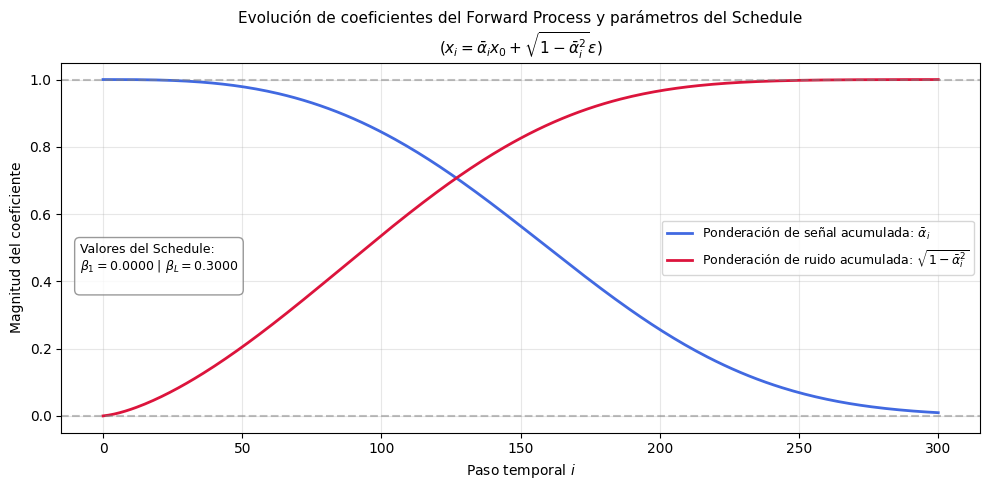
\includegraphics[width=\textwidth]{Aux/02_2_DDPM/NoiseSchedule.png}
        \caption{Ejemplo de schedule de ruido.}
        \label{fig:noise_schedule}
        \vspace{-1em}
        {\tiny \color{gray} Fuente: Autoría propia~\cite{DDPM-MNIST}.}
    \end{figure}
\end{frame}

\begin{frame}{Ejemplo de Forward Process}
    \begin{figure}
        \centering
        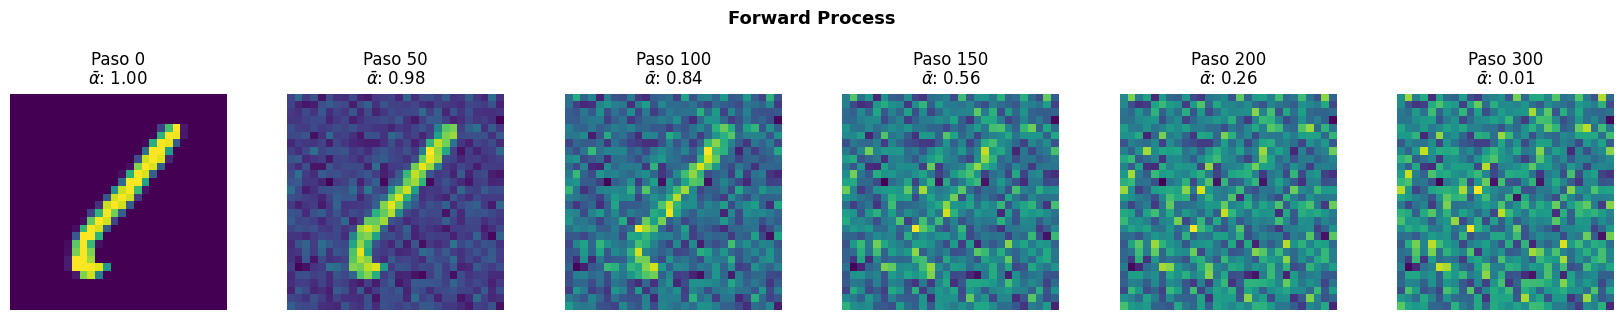
\includegraphics[width=\textwidth]{Aux/02_2_DDPM/ForwardPass.png}
        \caption{Ejemplo de Forward Process.}
        \label{fig:forward_pass}
        \vspace{-1em}
        {\tiny \color{gray} Fuente: Autoría propia~\cite{DDPM-MNIST}.}
    \end{figure}
\end{frame}


\section{Reverse Process}

\begin{frame}
    \frametitle{Reverse Process}
    
    Proceso \emph{aprendido} que transforma un dato ruidoso $\mathbf{x}_L\sim \mathcal{N}(\mathbf{0}, \mathbf{I})$ en un dato original $\mathbf{x}_0$ a través de $L$ pasos de difusión inversa.
    \pause
    Por la Regla de Bayes, la distribución de $x_{i-1}$ dado $x_i$ es:
    \begin{equation*}
        p_{i}(x_{i-1}|x_i) = \frac{p_i(x_i|x_{i-1}) p_{i-1}(x_{i-1})}{p_i(x_i)}
        \qquad
        p_i(x_i) = \int p_i(x_i|x_0)p_{\text{data}}(x_0)\ dx_0
    \end{equation*}
    \pause
    \begin{center}
        \large{\alt<5>{{\color{red}¡Intractable!}}{¡Intractable!}}
    \end{center}
    \pause
    Se aproxima $p_i(x_{i-1}|x_i)$ empleando una red neuronal $p_{{\phi}}(x_{i-1}|x_i)$, que se entrena para minimizar la divergencia KL entre ambas distribuciones.
    \begin{equation*}
        \phi^* = \arg\min_{\phi} \mathbb{E}_{x_i\sim p_i(x_i)} \left[ \cc{D}_{\text{KL}}\left(p_i(x_{i-1}|x_i) || p_{\phi}(x_{i-1}|x_i)\right) \right]
    \end{equation*}
    \pause
\end{frame}


\begin{frame}[allowframebreaks]{Solución: Condicionar a $x_0$}
    \begin{lemma}
        Al condicionar $p_i(x_{i-1}|x_i)$ a $x_0$, el resultado es una distribución gaussiana:
        \begin{equation*}
            p_i(x_{i-1}|x_i, x_0) = \mathcal{N}\left(x_{i-1}; {\mu}_i(x_i, x_0, i), \sigma^2(i) \mathbf{I}\right)
        \end{equation*}
        donde:
        \begin{equation*}
            {\mu}_i(x_i, x_0, i) = \frac{{\bar{\alpha}_{i-1}}\beta_i^2}{1 -\bar{\alpha}_i^2} x_0 + \frac{{\alpha_i}(1 - \bar{\alpha}_{i-1}^2)}{1 - \bar{\alpha}_i^2} x_i, \quad \sigma(i)^2 = \frac{1 - \bar{\alpha}_{i-1}^2}{1 - \bar{\alpha}_i^2} \beta_i^2
        \end{equation*}
    \end{lemma}
    \pause
    \begin{theorem}
        \begin{multline*}
            \mathbb{E}_{p_i(x_i)} \left[ \cc{D}_{\text{KL}}\left(p_i(x_{i-1}|x_i) || p_{\phi}(x_{i-1}|x_i)\right) \right] =\\= \mathbb{E}_{p_{\text{data}}(x_0)} \mathbb{E}_{p_i(x_i|x_0)} \left[ \cc{D}_{\text{KL}}\left(p_i(x_{i-1}|x_i, x_0) || p_{\phi}(x_{i-1}|x_i)\right) \right] + C
        \end{multline*}
        donde $C$ es una constante independiente de $\phi$.
    \end{theorem}
\end{frame}

\begin{frame}{Ejemplo de Reverse Process}
    \begin{figure}
        \centering
        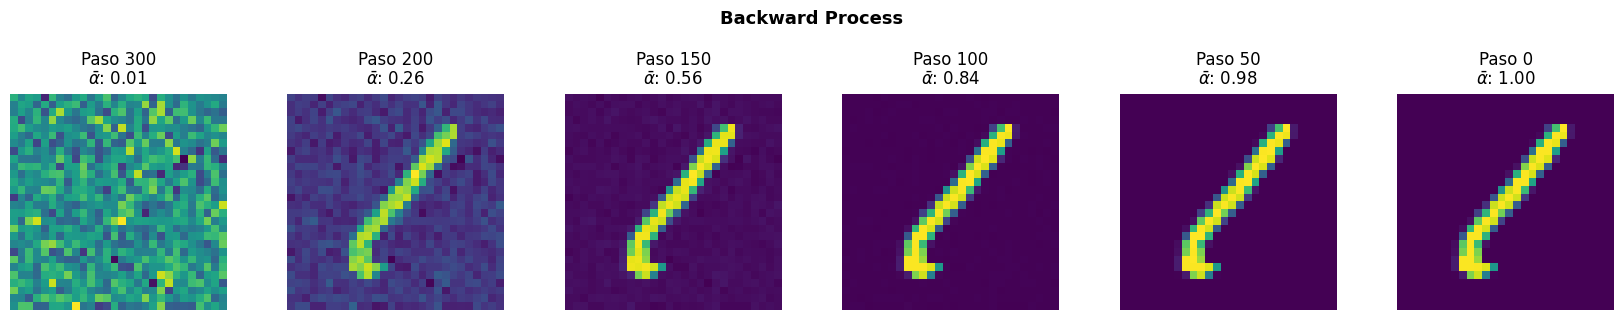
\includegraphics[width=\textwidth]{Aux/02_2_DDPM/ReversePass.png}
        \caption{Ejemplo de Reverse Process.}
        \label{fig:reverse_pass}
        \vspace{-1em}
        {\tiny \color{gray} Fuente: Autoría propia~\cite{DDPM-MNIST}.}
    \end{figure}
\end{frame}


\begin{frame}{Modelado de Red Neuronal}
    Siguiendo el lema anterior, se modela $p_{\phi}(x_{i-1}|x_i)$ como una distribución gaussiana:
    \begin{equation*}
        p_{\phi}(x_{i-1}|x_i) = \mathcal{N}\left(x_{i-1}; {\mu}_{\phi}(x_i, i), \sigma^2(i) \mathbf{I}\right)
    \end{equation*}
    donde $\sigma^2(i)$ es el valor de la varianza anteriormente descrito y ${\mu}_{\phi}(\cdot, i): \mathbb{R}^d \to \mathbb{R}^d$ es una red neuronal que aproxima ${\mu}_i(x_i, x_0, i)$.
\end{frame}

\begin{frame}{Función de Pérdida}
    La función de pérdida a minimizar es la divergencia KL entre las distribuciones gaussianas:
    \begin{align*}
        \mathcal{L}_{\text{DDPM}}(\phi) &= \sum_{i=2}^{L} \mathbb{E}_{p_{\text{data}}(x_0)} \mathbb{E}_{p_i(x_i|x_0)} \left[ \mathcal{D}_{\text{KL}}\left(p_i(x_{i-1}|x_i, x_0) \parallel p_{\phi}(x_{i-1}|x_i)\right) \right] \\
        \visible<2->{&= \sum_{i=2}^{L} \frac{1}{2\sigma^2(i)} \mathbb{E}_{p_{\text{data}}(x_0)} \mathbb{E}_{p_i(x_i|x_0)} \left[ \left\| \boldsymbol{\mu}(x_i, x_0, i) - \boldsymbol{\mu}_{\phi}(x_i, i) \right\|^2 \right] + C}
    \end{align*}
    \visible<2->{donde $C$ es una constante independiente de $\phi$.}
\end{frame}

\begin{frame}{Monte Carlo como Estimador Insesgado}
    Al tratarse el estimador de Monte Carlo de un {\color{red}estimador insesgado}, se puede reescribir la función de pérdida como:
    \begin{equation*}
        (L-1) \bb{E}_{i\sim\cc{U}\{2,\dots,L\}} \mathbb{E}_{p_{\text{data}}(x_0)} \mathbb{E}_{p_i(x_i|x_0)} \left[ \frac{1}{2\sigma^2(i)} \left\| \boldsymbol{\mu}(x_i, x_0, i) - \boldsymbol{\mu}_{\phi}(x_i, i) \right\|^2 \right] + C
    \end{equation*}
    \pause
    A efectos de entrenamiento, se puede reescribir la función de pérdida como:
    \begin{equation*}
        \mathbb{E}_{i\sim\cc{U}\{2,\dots,L\}} \mathbb{E}_{p_{\text{data}}(x_0)} \mathbb{E}_{p_i(x_i|x_0)} \left[ \frac{1}{2\sigma^2(i)} \left\| \boldsymbol{\mu}(x_i, x_0, i) - \boldsymbol{\mu}_{\phi}(x_i, i) \right\|^2 \right]
    \end{equation*}
    
\end{frame}


\begin{frame}{Problema: Desbordamiento}
    Debido a los valores muy pequeños de $\sigma^2(i)$, la función de pérdida se desborda.
    \begin{figure}
        \centering
        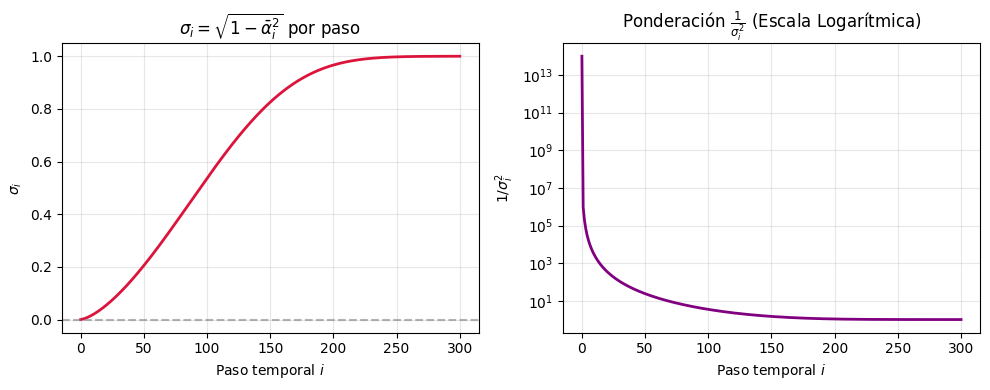
\includegraphics[width=\textwidth]{Aux/02_2_DDPM/Desbordamiento.png}
        \caption{Valores de $\sigma^2(i)$ para un ejemplo de schedule de ruido.}
        \label{fig:desbordamiento}
        \vspace{-1em}
        {\tiny \color{gray} Fuente: Autoría propia~\cite{DDPM-MNIST}.}
    \end{figure}
\end{frame}



\begin{frame}{$\epsilon$-Prediction}
    En lugar de predecir $\mu_\phi(x_i, i)$, se predice $\epsilon_\phi(x_i, i)$, el ruido añadido en el paso $i$, puesto que:
    \begin{equation*}
        \mu_i(x_i, x_0, i) = \frac{1}{\alpha_i} \left( x_i - \frac{\beta_i^2}{\bar{\beta}_i} \epsilon \right) \implies \mu_\phi(x_i, i) = \frac{1}{\alpha_i} \left( x_i - \frac{\beta_i^2}{\bar{\beta}_i} \epsilon_\phi(x_i, i) \right)
    \end{equation*}
    donde $\bar{\beta}_i^2+\bar{\alpha}_i^2 = 1$.
    \pause
    La función de pérdida se reescribe como:
    \begin{equation*}
        \mathbb{E}_{i\sim\cc{U}\{2,\dots,L\}} \mathbb{E}_{p_{\text{data}}(x_0)} \mathbb{E}_{\epsilon\sim \cc{N}(0,\mathbf{I})} \left[ w(i) \left\| \epsilon - \epsilon_\phi(x_i, i) \right\|^2 \right]
    \end{equation*}
    donde $w(i)$ es un factor de peso.
    \pause
    Puesto que $\epsilon\sim \cc{N}(0,\mathbf{I})$, la diferencia $\epsilon - \epsilon_\phi(x_i, i)$ es de magnitud similar para todos los pasos $i$, por lo que el factor de peso $w(i)$ puede eliminarse\footnote{Esto no ocurría en el caso de \emph{mean}-prediction.}, obteniéndose la función de pérdida final:
    \begin{equation*}
        \mathcal{L}_{\text{DDPM}}(\phi) = \mathbb{E}_{i\sim\cc{U}\{2,\dots,L\}} \mathbb{E}_{p_{\text{data}}(x_0)} \mathbb{E}_{\epsilon\sim \cc{N}(0,\mathbf{I})} \left[ \left\| \epsilon - \epsilon_\phi(x_i, i) \right\|^2 \right]
    \end{equation*}
\end{frame}


\begin{frame}{$x_0$-Prediction}
    En lugar de predecir $\mu_\phi(x_i, i)$ o $\epsilon_\phi(x_i, i)$, se predice $x_{0,\phi}(x_i, i)$, el dato original a partir del dato ruidoso en el paso $i$, puesto que:
    \begin{equation*}
        {\mu_\phi}_i(x_i, i) = \frac{{\bar{\alpha}_{i-1}}\beta_i^2}{1 -\bar{\alpha}_i^2} x_{0,\phi}(x_i, i) + \frac{{\alpha_i}(1 - \bar{\alpha}_{i-1}^2)}{1 - \bar{\alpha}_i^2} x_i
    \end{equation*}
    \pause
    La función de pérdida se reescribe como:
    \begin{equation*}
        \mathbb{E}_{i\sim\cc{U}\{2,\dots,L\}} \mathbb{E}_{p_{\text{data}}(x_0)} \mathbb{E}_{\epsilon\sim \cc{N}(0,\mathbf{I})} \left[ w(i) \left\| x_0 - x_{0,\phi}(x_i, i) \right\|^2 \right]
    \end{equation*}
    donde $w(i)$ es un factor de peso.
    \pause
    Puesto que $x_0$ es de magnitud similar para todos los pasos $i$, el factor de peso $w(i)$ puede eliminarse, obteniéndose la función de pérdida final:
    \begin{equation*}
        \mathcal{L}_{\text{DDPM}}(\phi) = \mathbb{E}_{i\sim\cc{U}\{2,\dots,L\}} \mathbb{E}_{p_{\text{data}}(x_0)} \mathbb{E}_{\epsilon\sim \cc{N}(0,\mathbf{I})} \left[ \left\| x_0 - x_{0,\phi}(x_i, i) \right\|^2 \right]
    \end{equation*}
    \pause    
\end{frame}

\section{ELBO de DDPM}

\begin{frame}{ELBO de DDPM}
    \begin{definitionblock}{ELBO de DDPM}
        El \emph{Evidence Lower Bound} (ELBO) de un DDPM es:
        \begin{equation*}
            \cc{L}_{\text{ELBO}}(\phi; x_0) = \cc{L}_{\text{prior}}(x_0) + \cc{L}_{\text{recon.}}(x_0; \phi) + \cc{L}_{\text{diffusion}}(x_0; \phi)
        \end{equation*}
        \begin{align*}
            \cc{L}_{\text{prior}}(x_0) &= \cc{D}_{\text{KL}}\left(p(x_L|x_0) \parallel p_{\text{prior}}(x_L)\right) \\
            \cc{L}_{\text{recon.}}(x_0; \phi) &= \mathbb{E}_{p(x_1|x_0)} \left[-\log p_\phi(x_0|x_1)\right] \\
            \cc{L}_{\text{diffusion}}(x_0; \phi) &= \sum_{i=2}^{L} \mathbb{E}_{p_i(x_i|x_0)} \left[\cc{D}_{\text{KL}}\left(p(x_{i-1}|x_i, x_0) \parallel p_\phi(x_{i-1}|x_i)\right)\right]
        \end{align*}
        
    \end{definitionblock}
\end{frame}
\begin{frame}{ELBO de DDPM}
    Se define:
    \begin{align*}
        p_\phi(x_0, x_{1:L}) &= p_\phi(x_0|x_1)p_\phi(x_1|x_2)\cdots p_\phi(x_{L-1}|x_L)p(x_L) \\
        \visible<2->{p_\phi(x_0) &= \int p_\phi(x_0, x_{1:L}) dx_{1:L}}
    \end{align*}
    \pause
    \begin{theorem}
        $$\log p_\phi(x_0) \geq \cc{L}_{\text{ELBO}}(\phi; x_0)$$
    \end{theorem}
\end{frame}

\section{Sampling}

\begin{frame}{Sampling}
    Una vez entrenado el modelo, se puede generar un dato original a partir de ruido puro:
    \begin{enumerate}
        \item Se genera un dato ruidoso $\mathbf{x}_L\sim \mathcal{N}(\mathbf{0}, \mathbf{I})$.
        \item Se aplica el Reverse Process, obteniéndose $\mathbf{x}_0$.
        \pause
        \begin{itemize}
            \item Si se ha entrenado el modelo para predecir $\mu_\phi(x_i, i)$:
            \begin{equation*}
                x_{i-1} = \mu_\phi(x_i, i) + \sigma(i) \epsilon, \quad \epsilon\sim\mathcal{N}(\mathbf{0}, \mathbf{I})
            \end{equation*}
            \pause
            \item Si se ha entrenado el modelo para predecir $\epsilon_\phi(x_i, i)$:
            \begin{equation*}
                \mu_\phi(x_i, i) = \frac{1}{\alpha_i} \left( x_i - \frac{\beta_i^2}{\bar{\beta}_i} \epsilon_\phi(x_i, i) \right)
            \end{equation*}
            \pause
            \item Si se ha entrenado el modelo para predecir $x_{0,\phi}(x_i, i)$:
            \begin{equation*}
                \epsilon_\phi(x_i, i) = \frac{x_i-\bar{\alpha}_i x_{0,\phi}(x_i, i)}{\bar{\beta}_i}
            \end{equation*}
        \end{itemize}
    \end{enumerate}
\end{frame}

\begin{frame}{Denoise y Re-noise}
    La predicción de $x_{i-1}$ a partir de $x_i$ cumple:
    \begin{equation*}
        \hat{x}_{i-1} = \bar{\alpha}_{i-1} x_{\phi^\times}(x_i, i) + \sqrt{1-\bar{\alpha}_{i-1}^2-\sigma^2(i)} \epsilon_{\phi^\times}(x_i, i) + \sigma(i) \epsilon, \quad \epsilon\sim\mathcal{N}(\mathbf{0}, \mathbf{I})
    \end{equation*}
    \pause

    Además, $(1-\bar{\alpha}_{i-1}^2-\sigma^2(i))+\sigma^2(i) = 1-\bar{\alpha}_{i-1}^2$, por lo que se puede entender que el proceso de predicción de $x_{i-1}$ a partir de $x_i$ consiste en:
    \begin{enumerate}
        \item \emph{Denoise}: Se elimina el ruido de $x_i$ para obtener $x_{0,\phi^\times}(x_i, i)$.
        \item \emph{Re-noise}: Se añade ruido a $x_{0,\phi^\times}(x_i, i)$ para obtener $\hat{x}_{i-1}$.
    \end{enumerate}
    \pause
    \begin{center}
        En el paso de \emph{Denoise}, solo se pueden predecir imágenes de \emph{media}, luego produce imágenes {\color{red}borrosas} (especialmente en pasos altos).
    \end{center}
\end{frame}

\begin{frame}{Baja velocidad de síntesis}
    Fijado un número de pasos $L$, la síntesis requiere $L$ pasos de predicción en los que cada uno depende del anterior. Esto provoca $\cc{O}(L)$ pasos de predicción, imposibilitando la paralelización de la síntesis.\vspace{0.5cm}

    \pause
    En nuestra aproximación, $p_{\phi}(x_{i-1}|x_i)$ es una gaussiana para aproximar $p_i(x_{i-1}|x_i)$, pera esta última no necesariamente es gaussiana (es mezcla ponderada de gaussianas).
    \begin{itemize}
        \item Si $beta_i$ es pequeño, $p_i(x_{i-1}|x_i)$ es unimodal y puede aproximarse bien con una gaussiana.
        \item Si $beta_i$ es grande, $p_i(x_{i-1}|x_i)$ puede ser multimodal y no puede aproximarse bien con una gaussiana.
    \end{itemize}
    
    Por tanto, se requiere un número grande de pasos $L$ para que $\beta_i$ sea pequeño y la aproximación sea buena, lo que provoca una \hspace{2cm} {\color{red}baja velocidad de síntesis}.    
\end{frame}




\begin{frame}[allowframebreaks]{Bibliografía}
    \nocite{lai2026principlesdiffusionmodels}
    \printbibliography
\end{frame}




\end{document}